\documentclass[conference]{IEEEtran}
\usepackage[T1]{fontenc}
\usepackage{graphicx}
\usepackage{cite}
\usepackage{amsmath}
\usepackage{amssymb}
\usepackage{hyperref}

\title{Overview Report: Deepening the Understanding of the Combination of Semantic Communication and Edge Intelligence}

\begin{document}

\maketitle

\begin{abstract}
This report provides an in-depth investigation into the integration of semantic communication (SemCom) with edge intelligence. Based on recent advances presented in relevant papers, it explores the underlying principles, technical challenges, and future research directions. Emphasizing deep analysis, this work critically evaluates how SemCom, enhanced by edge computing paradigms such as federated learning, can revolutionize resource efficiency, security, and scalability. Finally, it discusses strategic insights for practical deployment, highlighting potential pathways for innovation and key open problems.
\end{abstract}

\begin{IEEEkeywords}
Semantic Communication, Edge Intelligence, Federated Learning, Resource Optimization, Deep Learning, Knowledge Graphs, Edge Computing, Future Networks.
\end{IEEEkeywords}

\section{Introduction}
With the development of information and communication technologies and AI, the "internet of everything" 
has been considered as one of the vital visions of 6G, wherein semantic communication and AI 
are two key enablers. However, limitations of Shannon's classic information theory 
call for new motivations for this revolution. Recent researches shed light on semantic communication --- a communication 
framework that emphasizes the understanding and meaning of transmitted 
information, which represents a promising avenue to achieve the trade-off between efficiency, 
privacy, and robustness \cite{a1, a2}. But many constraints such as resource-limited end devices 
still hinder the scalable implementation of SemCom systems.

So, this report synthesizes insights from paper \cite{a3}, aiming to provide a profound understanding of the integration of Semantic communication and edge intelligence.

\section{Background and Motivation}
Traditional communication theories focus primarily on transmitting data reliably over 
noisy channels. However, in applications such as internet of things (IoT), the objective 
extends beyond data transmission: it encompasses the understanding of 
semantics, context, and goals.

\subsection{Semantic Communication Paradigm}
SemCom shifts the focus from bit-level transmission to meaning-level understanding \cite{a4}. Its core principles include:
\begin{itemize}
    \item \textbf{Semantic Encoding}: Compressing relevant information based on its meaning rather than raw data.
    \item \textbf{Semantic Decoding}: Reconstructing intended meaning effectively at the receiver.
    \item \textbf{Semantic Extraction}: Utilizing AI techniques like deep learning to extract semantic features.
\end{itemize}

\begin{figure}[h]
\centering
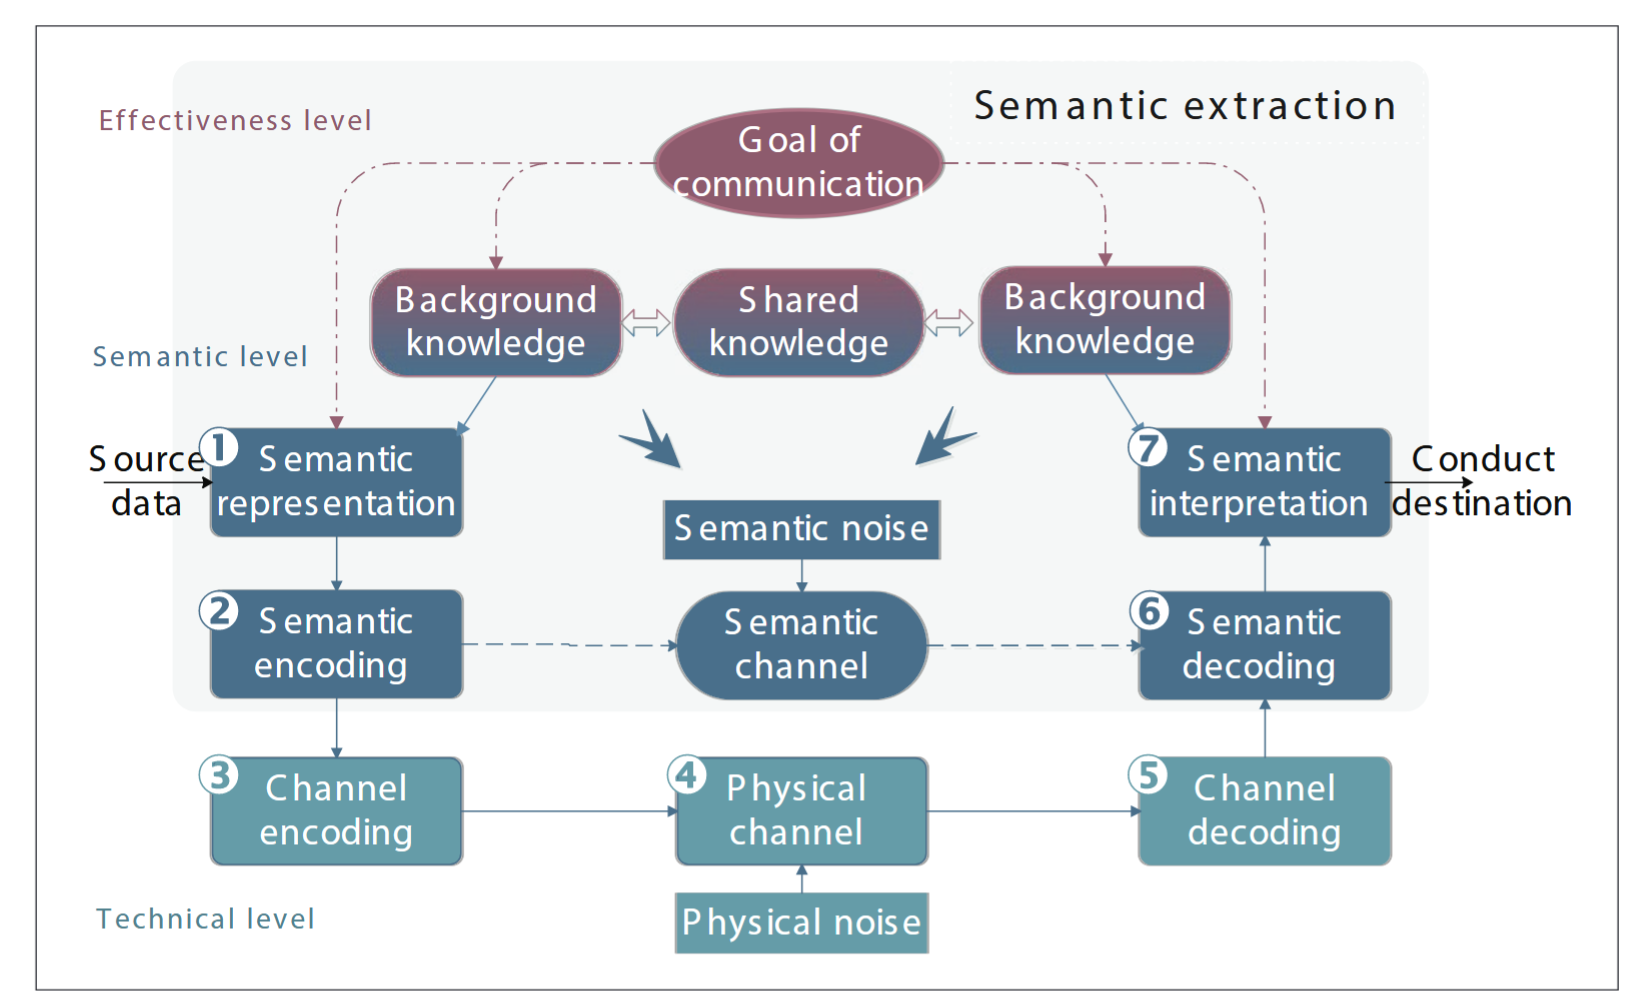
\includegraphics[width=0.45\textwidth]{fig-1.png}
\caption{SemCom model}
\end{figure}

\subsection{Edge Intelligence}
Edge computing distributes processing resources closer to data sources, reducing 
latency and improving security. When combined with AI techniques, 
it provides an environment where semantic models can be trained, updated, and 
deployed efficiently \cite{a5}.

\section{Semantic Communication Meets Edge Intelligence}
\subsection{Core Concepts and Techniques}
Based on the paper \textit{Semantic Communication Meets Edge Intelligence}, 
the integration depends on several advanced components:
\begin{itemize}
    \item \textbf{Semantic Extraction Techniques}: Utilizing deep neural networks, reinforcement learning, knowledge graphs, and semantic-native models to parse and encode meaning.
    \item \textbf{Distributed Learning}: Federated learning facilitates collaborative model training across edge devices without raw data sharing, addressing privacy concerns \cite{a6}.
    \item \textbf{Knowledge Graphs (KG)}: Leveraged for contextual understanding and semantic reasoning across distributed systems.
    \item \textbf{Semantic-Aware Resource Allocation}: Mechanisms such as auction-based algorithms optimize energy and spectrum usage based on semantic importance.
\end{itemize}

\subsection{Challenges and Constraints}
Despite promising prospects, several issues hinder practical deployment:
\begin{itemize}
    \item \textbf{Computational Oberheads}: Deep models for semantic extraction demand significant resources, incompatible with lightweight devices.
    \item \textbf{Model Generalization}: Ensuring models work efficiently across diverse edge devices and evolving environments remains difficult.
    \item \textbf{Privacy and Security}: While federated learning reduces raw data sharing, semantic security requires more robust solutions.
    \item \textbf{Interpretability}: Deep semantic models often act as Black Boxes, lacking powerful validation.
\end{itemize}

\section{Deep Analysis of the Integrated Framework}
\subsection{System Architecture}
Combining SemCom and edge intelligence, a layered architecture is constructed (Fig. \ref{fig:architecture}):
\begin{itemize}
    \item \textbf{Perception Layer}: IoT devices capture raw data.
    \item \textbf{Edge Layer}: Performs semantic encoding, local inference, and learning.
    \item \textbf{Cloud/Global Layer}: Coordinates global model updates, knowledge sharing, and reasoning.
\end{itemize}

This multi-layer paradigm enhances resource efficiency by transmitting only 
semantically relevant information, reducing bandwidth, and enabling real-time processing.

\begin{figure}[h]
\centering
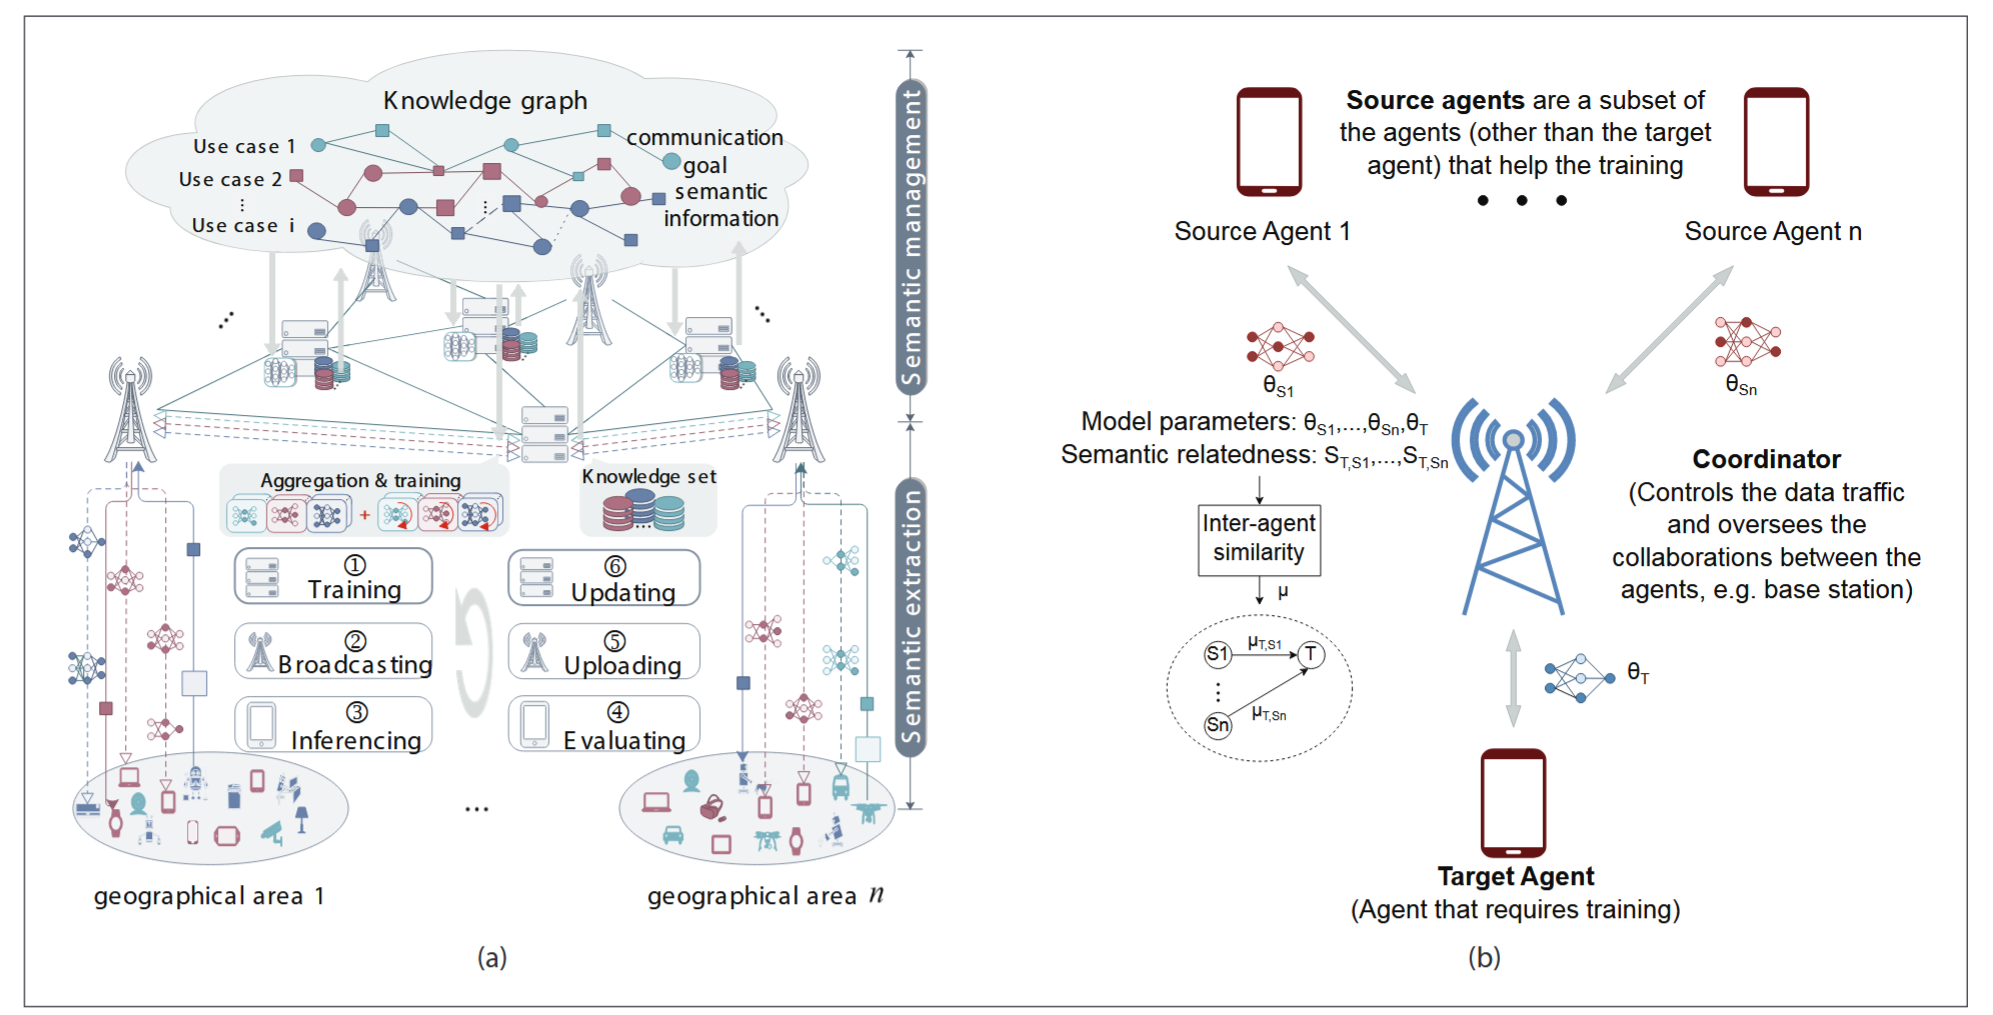
\includegraphics[width=0.45\textwidth]{fig-2.png}
\caption{Hierarchical edge-semantic communication architecture}
\label{fig:architecture}
\end{figure}

\subsection{Edge-Enabled SemCom}
The \textit{understand-before-transmission} paradigm of SemCom poses new challenges as follows:
\begin{itemize}
    \item Bandwidth cost and privacy loss.
    \item Computationally inefficient training.
    \item Long latency in training and updating SE models.
\end{itemize}

To address these challenges, an edge-enabled SemCom architecture is proposed.

Federated learning allows edge devices to collaboratively train models, preserving privacy \cite{a6}. 
With FL, the trained SE model parameters in edge servers can be exchanged 
directly with other edge servers with the identical tasks to accelerate the 
training process, improving the generalization performance of the model in a 
privacy-preserving manner.

In addition, a knowledge graph (KG) is leveraged to encode relations between 
communication goals and features, reducing computational and bandwidth costs.

\subsection{Semantic-Aware Edge Intelligence}
Deep reinforcement learning allows the intelligent agents to learn adaptively 
based on their own experiences. However, it may induce overfitting issues, 
long convergence time, and sub-optimal performance of the model. To tackle with 
these disadvantages, collaborative DRL is proposed to generalize the model 
experience by exchanging their model parameters or policies.

However, a drawback of CDRL and distributed deep learning is the high communication overheads 
incurred for exchanging model parameters. So model compression techniques are considered 
to foster the implementation of edge intelligence, which include:
\begin{itemize}
    \item \textbf{Gradient Sparsification}
    \item \textbf{Model Pruning}
\end{itemize}

\section{Case Study}
\subsection{Challenges}
Traditional resource allocation maximizes throughput without considering 
semantic importance or conflicting user-edge goals.

\subsection{Proposed Approaches}
To facilitate the convergence of SemCom and edge intelligence, the following approaches 
are adopted in the case study:
\begin{itemize}
    \item Redesign energy and data allocation policies to maximize semantic performance.
    \item Use an auction-based mechanism where IoT devices bid for energy based on expected semantic gains (sentence similarity, BLEU score).
    \item Allocate energy to devices that provide the highest semantic value, ensuring effective SemCom.
\end{itemize}

\subsection{System Model}
A system model in which energy-constraint IoT devices harvest the energy wirelessly 
for text transmission is proposed. Key procedures include:
\begin{itemize}
    \item Wireless-powered IoT devices encode/decode semantic information from text data.
    \item Devices bid for energy.
    \item The hybrid access point (HAP) determines winners via a DL-based auction.
    \item Devices adjust output dimensions based on energy constraints.
\end{itemize}

\begin{figure}[h]
\centering
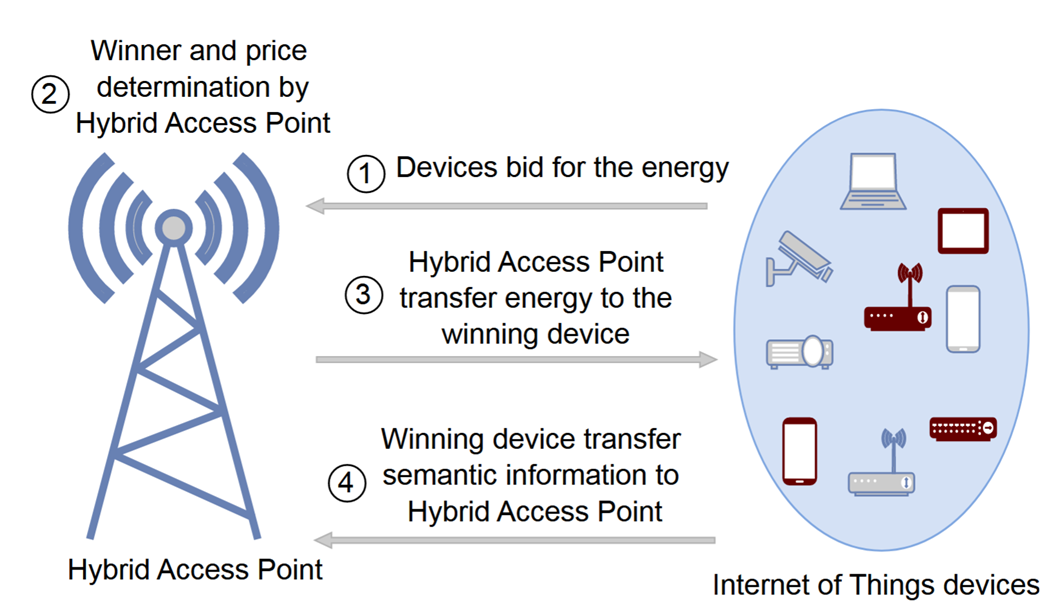
\includegraphics[width=0.45\textwidth]{fig-3.png}
\caption{System model of the case study}
\end{figure}

\subsection{Results}
\begin{itemize}
    \item Higher semantic quality (sentence similarity, BLEU score) leads to higher bids and better energy allocation.
    \item DL auction achieves higher revenue compared to traditional methods, effectively aligning resource distribution with semantic importance.
\end{itemize}

\begin{figure}[h]
\centering
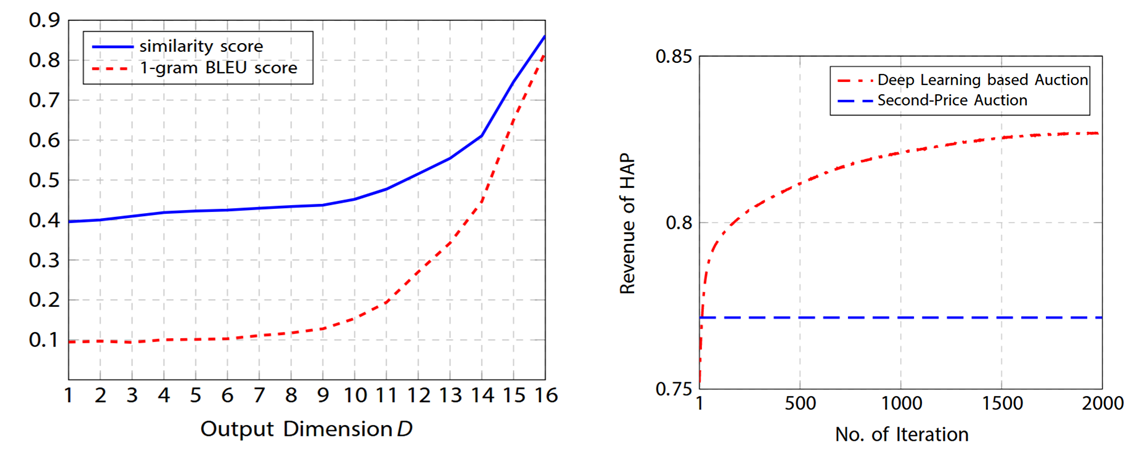
\includegraphics[width=0.45\textwidth]{fig-4.png}
\caption{Results of the case study}
\end{figure}

\section{Discussion and Critical Perspectives}
The convergence of SemCom and edge intelligence is revolutionary, offering tangible benefits like:
\begin{itemize}
    \item \textbf{Enhanced Efficiency}: Transmitting semantically relevant content rather than raw data reduces bandwidth and energy consumption.
    \item \textbf{Improved Privacy}: Local semantic modeling decreases raw data sharing.
    \item \textbf{Context-aware Communication}: Facilitates intelligent interactions in complex environments.
\end{itemize}

Yet, the field requires further refinements:
\begin{itemize}
    \item \textbf{Balancing Performance and Complexity}: Simplify semantic models without significantly losing accuracy.
    \item \textbf{Interoperability and Standardization}: Develop universal semantic protocols.
    \item \textbf{Explainability}: Build transparent models to foster trust in critical applications.
\end{itemize}

These issues underline that while technological advancements are promising, aligning research innovations with real-world constraints remains challenging.

\section{Future Directions and Concluding Remarks}
Emerging research areas to prioritize include:
\begin{itemize}
    \item \textbf{Interpretability and Explainability of SE}
    \item \textbf{Semantic Privacy and Security}
    \item \textbf{Variable-Length Semantic Encoding}
    \item \textbf{DL-Based Task Similarity Measurement}
    \item \textbf{Semantic Compression of Model Parameters}
\end{itemize}

\subsection{Key Takeaways}
\begin{itemize}
    \item Semantic communication combined with edge intelligence can reshape the efficiency and security of 6G networks.
    \item Leveraging AI techniques like deep learning, knowledge graphs, and federated learning is central to this evolution.
    \item Addressing computational, privacy, and interpretability challenges is vital for real-world deployment.
    \item Innovative architectures and adaptive models will define the future landscape of intelligent, semantic-aware next-generation networks.
\end{itemize}

\subsection{Conclusion}
Semantic communication at the edge bears immense potential but demands meticulous research to solve underlying challenges. Its success will depend on interdisciplinary convergence—integrating AI, communications, security, and human-centric design.

\begin{thebibliography}{1}

\bibitem{a1} S. Chen et al., "Semantic communication: Concepts, challenges, and future directions," \textit{IEEE Wireless Communications}, vol. 28, no. 2, pp. 157-163, 2021.
\bibitem{a2} Z. Yang et al., "Semantic-aware edge learning for next-generation wireless networks," \textit{IEEE Communications Magazine}, vol. 59, no. 7, pp. 88-94, 2021.
\bibitem{a3} W. Yang et al., "Semantic Communication Meets Edge Intelligence," \textit{IEEE Wireless Communications}, vol. 29, no. 5, pp. 28-35, October 2022.
\bibitem{a4} T. Liu et al., "Deep semantic encoding for wireless communications," \textit{IEEE Journal on Selected Areas in Communications}, vol. 40, no. 6, pp. 1708-1724, 2022.
\bibitem{a5} H. Zhang et al., "Edge intelligence for 6G: Paradigms, architectures, and applications," \textit{IEEE Wireless Communications}, vol. 29, no. 2, pp. 6-13, 2022.
\bibitem{a6} Q. Yang et al., "Federated learning: A survey on techniques, applications, and open issues," \textit{IEEE Transactions on Neural Networks and Learning Systems}, vol. 29, no. 1, pp. 78-89, 2022.
\end{thebibliography}

\end{document}
